\chapter{Lagebeziehungen}
\begin{inhalt}
  Wie liegen zueinander:
  \begin{itemize}
    \item Punkt-Gerade, Punkt-Ebene
    \item Gerade-Gerade, Gerade-Ebene
    \item Ebene-Ebene
  \end{itemize}
\end{inhalt}

\begin{bla}{Punktproben}
  Um zu sehen ob ein Punkt auf einer Geraden oder Ebene liegt, setzt man seine Koordinaten in deren Gleichungen ein.
  Es ergibt sich entweder eine wahre Aussage ($0=0$ - Punkt liegt auf der Geraden) oder eine falsche ($10 = 10.5$ - Punkt liegt nicht auf der Geraden)
\end{bla}

\begin{bla}{Gerade - Gerade}
  \begin{align*}
    \text{g: }\ \vec{x} &= \vec{p} + r * \vec{u} \\
    \text{h: }\ \vec{x} &= \vec{q} + s * \vec{v}
  \intertext{Man sucht Punkte, die auf beiden Geraden liegen.
  Dazu setzt man das $\vec{x}$ der beiden gleich.
  Man erhält ein LGS für die beiden Parameter:}
    \vec{p} + r * \vec{u} &= \vec{q} + s * \vec{v}
\end{align*}
  Sucht man jetzt Lösungen für $r$ und $s$, kann man folgende Ergebnisse bekommen:
  %
  \begin{marginfigure}[-10em]
    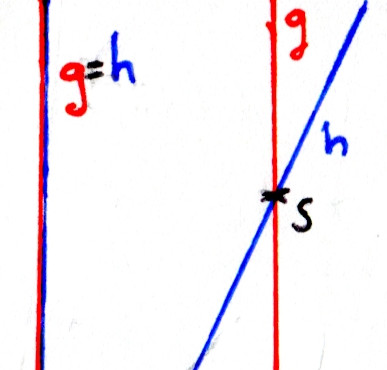
\includegraphics[scale=0.8]{AGLage_GerGerKontakt}
    \caption{Sich berührende Geraden}
  \end{marginfigure}
  %
  %
  \begin{marginfigure}[0em]
    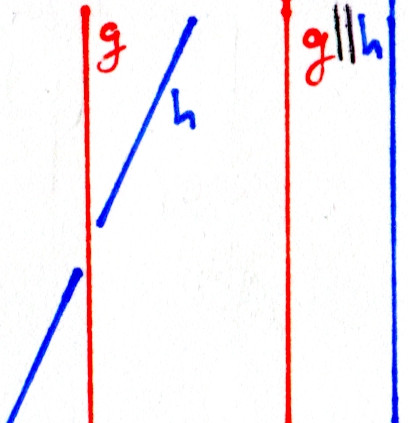
\includegraphics[scale=0.8]{AGLage_GerGerVorbei}
    \caption{Sich nicht berührende Geraden}
  \end{marginfigure}
  %
  \begin{itemize}
    \item $\infty$ \textbf{Lösungen}: Die Geraden sind \emph{identisch}.
    \item \textbf{Eine Lösung}: Es gibt einen \emph{Schnittpunkt} S.
    Er wird berechnet, indem man die Lösung für $k$ oder $l$ in die jeweilige Geradengleichung einsetzt.
    \item \textbf{Keine Lösung}: Die Geraden sind \emph{parallel} wenn die Richtungsvektoren linear abhängig sind.
    Wenn nicht, nennt man sie \emph{windschief}.
  \end{itemize}
\end{bla}

\begin{bla}{Gerade - Ebene}
  \label{AG_LageGE}
  Man setzt die Geradengleichung in die Ebenengleichung ein:
  \begin{align*}
    \text{g: }\ &\vec{x} = \vec{p} + \text{k} * \vec{u}
    \\
    \text{E: }\ &n_1x_1 + n_2x_2 + n_3x_3 = b
    \intertext{Das $\vec{x}$ aus g wird in E eingesetzt:}
    n_1(p_1 + k * u_1) + &n_2(p_2 + k * u_2) + n_3(p_3 + k * u_3) = b
  \end{align*}
  Alles bis auf k ist bekannt.
  Wie oben gibt es wieder verschiedene Lösungen für k:
  %
  \begin{marginfigure}[-30em]
    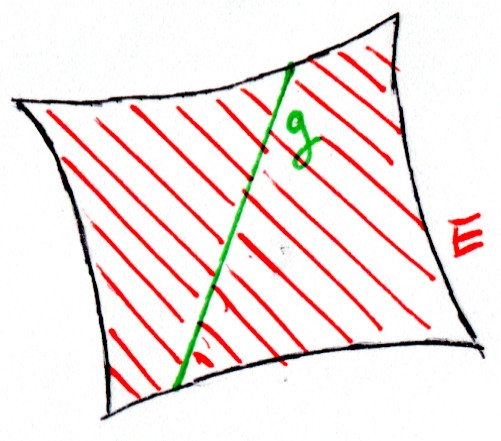
\includegraphics[scale=0.8]{AGAbstand_EbGerIdentisch}
    \caption{Gerade die in einer Ebene verläuft}
  \end{marginfigure}
  %
  %
  \begin{marginfigure}[-7.3em]
    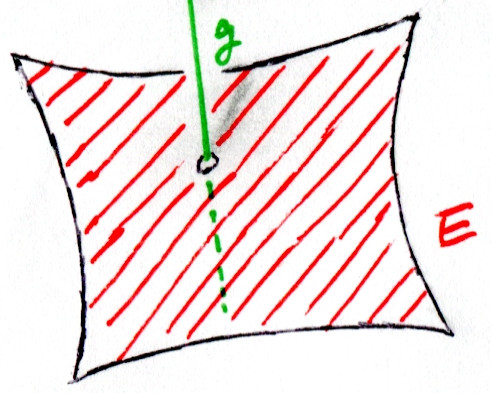
\includegraphics[scale=0.8]{AGAbstand_EbGerSchnitt}
    \caption{Gerade schneidet Ebene}
  \end{marginfigure}
  %
  %
  \begin{marginfigure}[0em]
    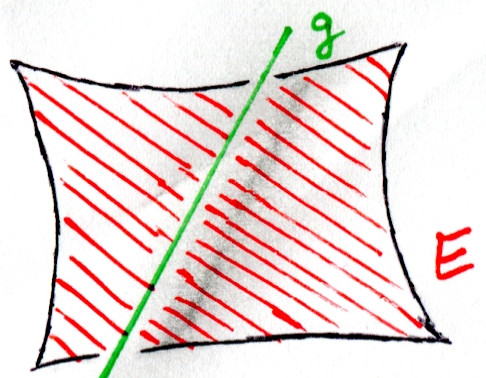
\includegraphics[scale=0.8]{AGAbstand_EbGerParallel}
    \caption{Gerade parallel zu Ebene}
  \end{marginfigure}
  %
  \begin{itemize}
    \item \textbf{Eine Lösung} ($k=2$): Es gibt einen \emph{Schnittpunkt} S.
    Er wird berechnet, indem man die Lösung für $k$ in die Geradengleichung einsetzt.
    \item \textbf{Wahre Aussage} ($1=1$): Die Gerade \emph{liegt in} der Ebene.
    \item \textbf{Widerspruch} ($1=27$): Gerade und Ebene sind \emph{parallel}.
  \end{itemize}
\end{bla}

\begin{bla}{Ebene - Ebene}
  Man setzt die $\vec{x}$ aus den Ebenengleichungen gleich und erhält ein LGS.
  %
  \begin{marginfigure}[0em]
    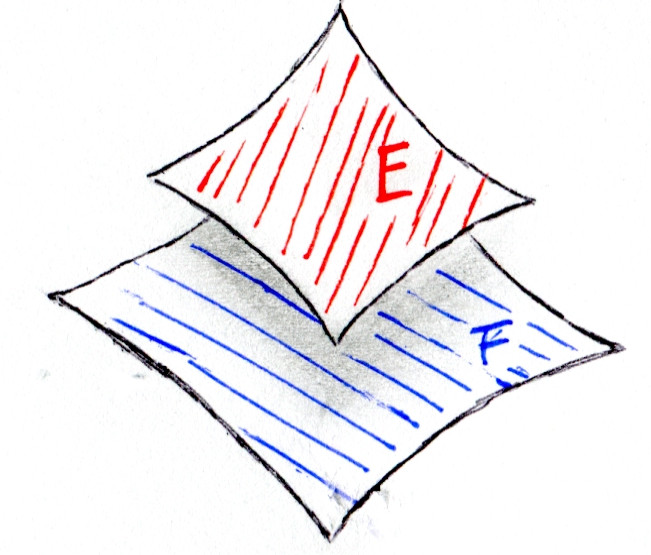
\includegraphics[scale=0.8]{AGLage_EbEbParallel}
    \caption{Parallele Ebenen}
  \end{marginfigure}
  %
  %
  \begin{marginfigure}[0em]
    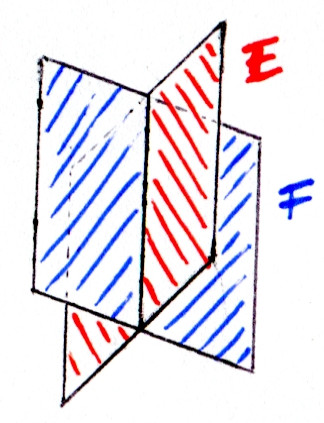
\includegraphics[scale=1.2]{AGLage_EbEbSchnitt}
    \caption{Ebenen mit Schnittgerade}
  \end{marginfigure}
  %
  \begin{itemize}
    \item Ergibt sich ein \textbf{Widerspruch}, so sind die Ebenen parallel.
    \item Ergibt sich eine \textbf{unendliche Lösung}, so liefert die Lösung die Schnittgerade der beiden Ebenen.
  \end{itemize}

  Hat man die Ebenen in Koordinaten- oder Normalenform vorliegen, so kann man auch die beiden Normalenvektoren in ein Kreuzprodukt schreiben.
  Das Ergebnis ist der Richtungsvektor der Schnittgeraden oder Null, falls die Ebenen parallel sind.
  Dann braucht man noch einen einzigen Stützpunkt, der in beiden Ebenen liegt und hat die Schnittgerade bestimmt.
\end{bla}
